\section{Auswertung}
\label{sec:Auswertung}

\subsection{Statische Methode}
\label{sec:auswertung_statisch}

Zur Auswertung der statischen Methode sollen zunächst die ausgedruckten Graphen
miteinander verglichen werden. Die Abbildungen \ref{fig:T1_T4} und \ref{fig:T5_T8} zeigen
die Temperaturen der verschiedenen Stäbe an den vom Peltier-Element weiter entfernten
Thermoelementen. Bei beiden Messingstäben, sowie bei dem Aluminiumstab kann ein annähernd
exponentieller Anstieg der Temperatur mit der Zeit erkannt werden. Die Graphen
zeigen zunächst einen Zuwachs der Steigung, steigen dann  steil an und flachen
gegen Ende der Messung leicht ab. Die Graphen unterscheiden sich jedoch in ihrer
Höhe und ihrer Steigung. Der Temperaturverlauf des Edelstahlstabes ist zunächst
konstant und zeigt nach etwa $40$\,s ein leichtes Wachstum der Steigung.

\begin{figure}
  \centering
  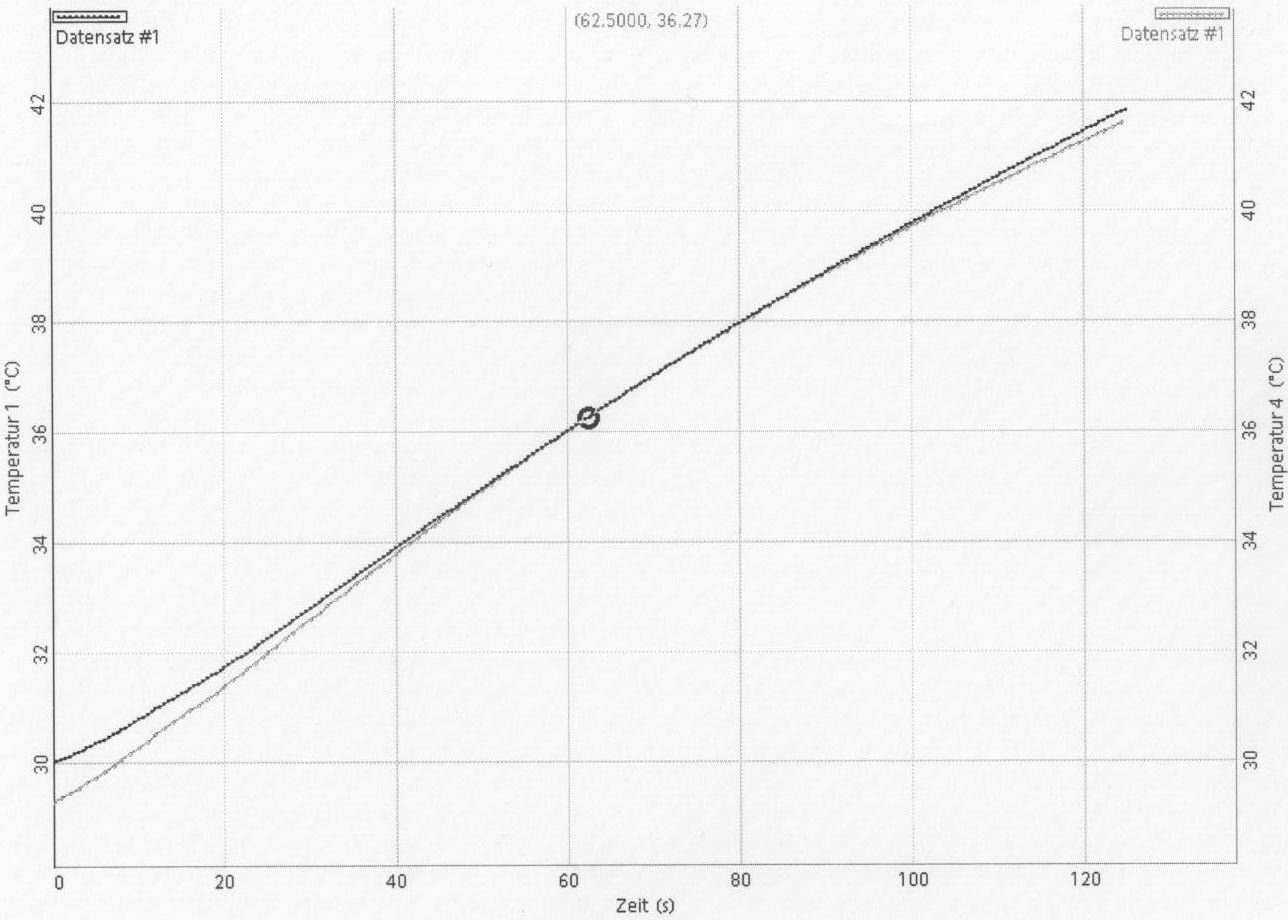
\includegraphics[width=0.7\textwidth]{data/t1undt4.JPEG}
  \caption{Temperaturverlauf des dicken Messingstabes (in der Abbildung dick dargestellt)
  und des dünnen Messingstabes (in der Abbildung dünn dargestellt) an den vom Peltier-
  Element weiter entfernten Themoelementen in Abhängigkeit von der Zeit}
  \label{fig:T1_T4}
\end{figure}

\begin{figure}
  \centering
  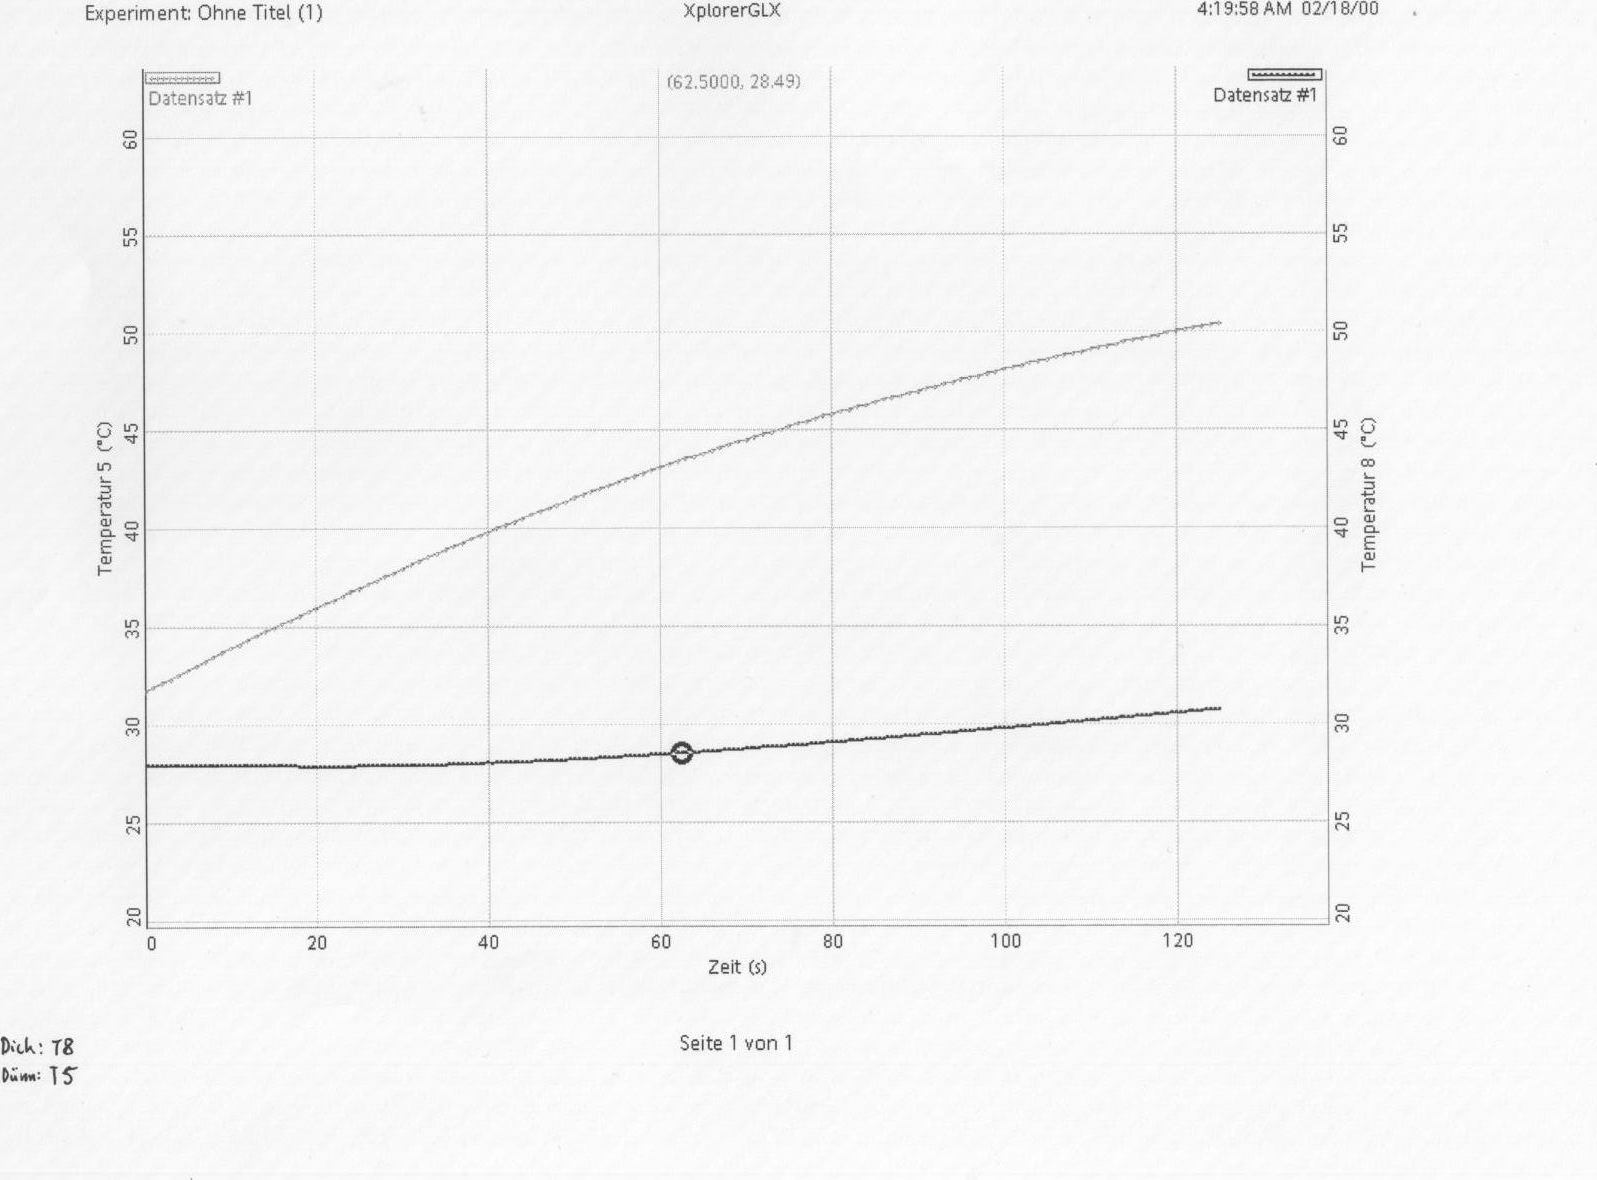
\includegraphics[width=0.7\textwidth]{data/t5undt8.JPEG}
  \caption{Temperaturverlauf des Aluminiumstabes (in der Abbildung dünn dargestellt)
  und des Edelstahlstabes (in der Abbildung dick dargestellt) an den vom Peltier-
  Element weiter entfernten Themoelementen in Abhängigkeit von der Zeit}
  \label{fig:T5_T8}
\end{figure}

Um festzustellen, welcher der Stäbe die beste Wärmeleitung besitzt, sollen die Temperaturen
der Stäbe nach $700$\,s abgelesen werden. Da die Messung jedoch auf Anweisung der Versuchsleitung
mit einem größeren Strom durchgeführt wurde, als in der Anleitung vermerkt, musste die Messung
bereits nach etwa $120$\,s abgebrochen werden, um ein Überhitzen der Stäbe zu vermeiden.
Daher werden an dieser Stelle die Temperaturen der verschiedenen Stäbe am Ende der
Messung verwendet. Diese betragen
\begin{align}
  T_1 &= \SI{314.95}{\kelvin}\,, \nonumber \\
  T_4 &= \SI{314.75}{\kelvin}\,,  \nonumber\\
  T_5 &= \SI{323.65}{\kelvin}\,,  \nonumber \\
  T_8 &= \SI{303.95}{\kelvin}\,.  \nonumber
\end{align}
Es ist erkennbar, dass der Aluminiumstab die höchste Temperatur besitzt. Da alle
Stäbe ungefähr die gleiche Ausgangstemperatur hatten, kann daraus geschlossen werden,
dass der Aluminiumstab die beste Wärmeleitung besitzt.

Nun soll der Verlauf der Temperaturdifferenzen am breiten Messingstab und am Edelstahlstab
in Abhängigkeit von der Zeit betrachtet werden. Die Verläufe sind in den Abbildungen
\ref{fig:Messing_diff} und \ref{fig:Stahl_diff} dargestellt.

\begin{figure}
  \centering
  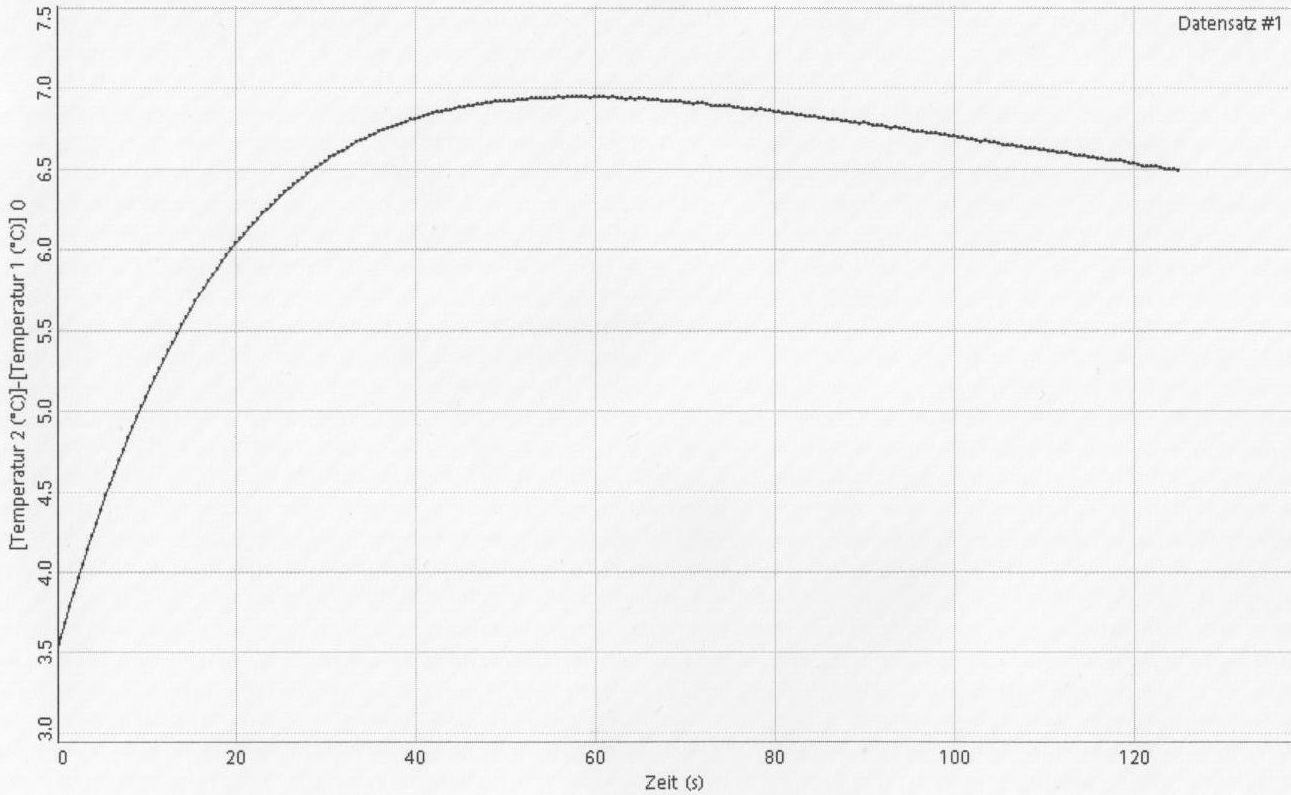
\includegraphics[width=0.7\textwidth]{data/t2minust1.JPEG}
  \caption{Verlauf der Temperaturdifferenz des fernen und des nahen Thermoelements am Messingstab
   in Abhängigkeit von der Zeit}
  \label{fig:Messing_diff}
\end{figure}

\begin{figure}
  \centering
  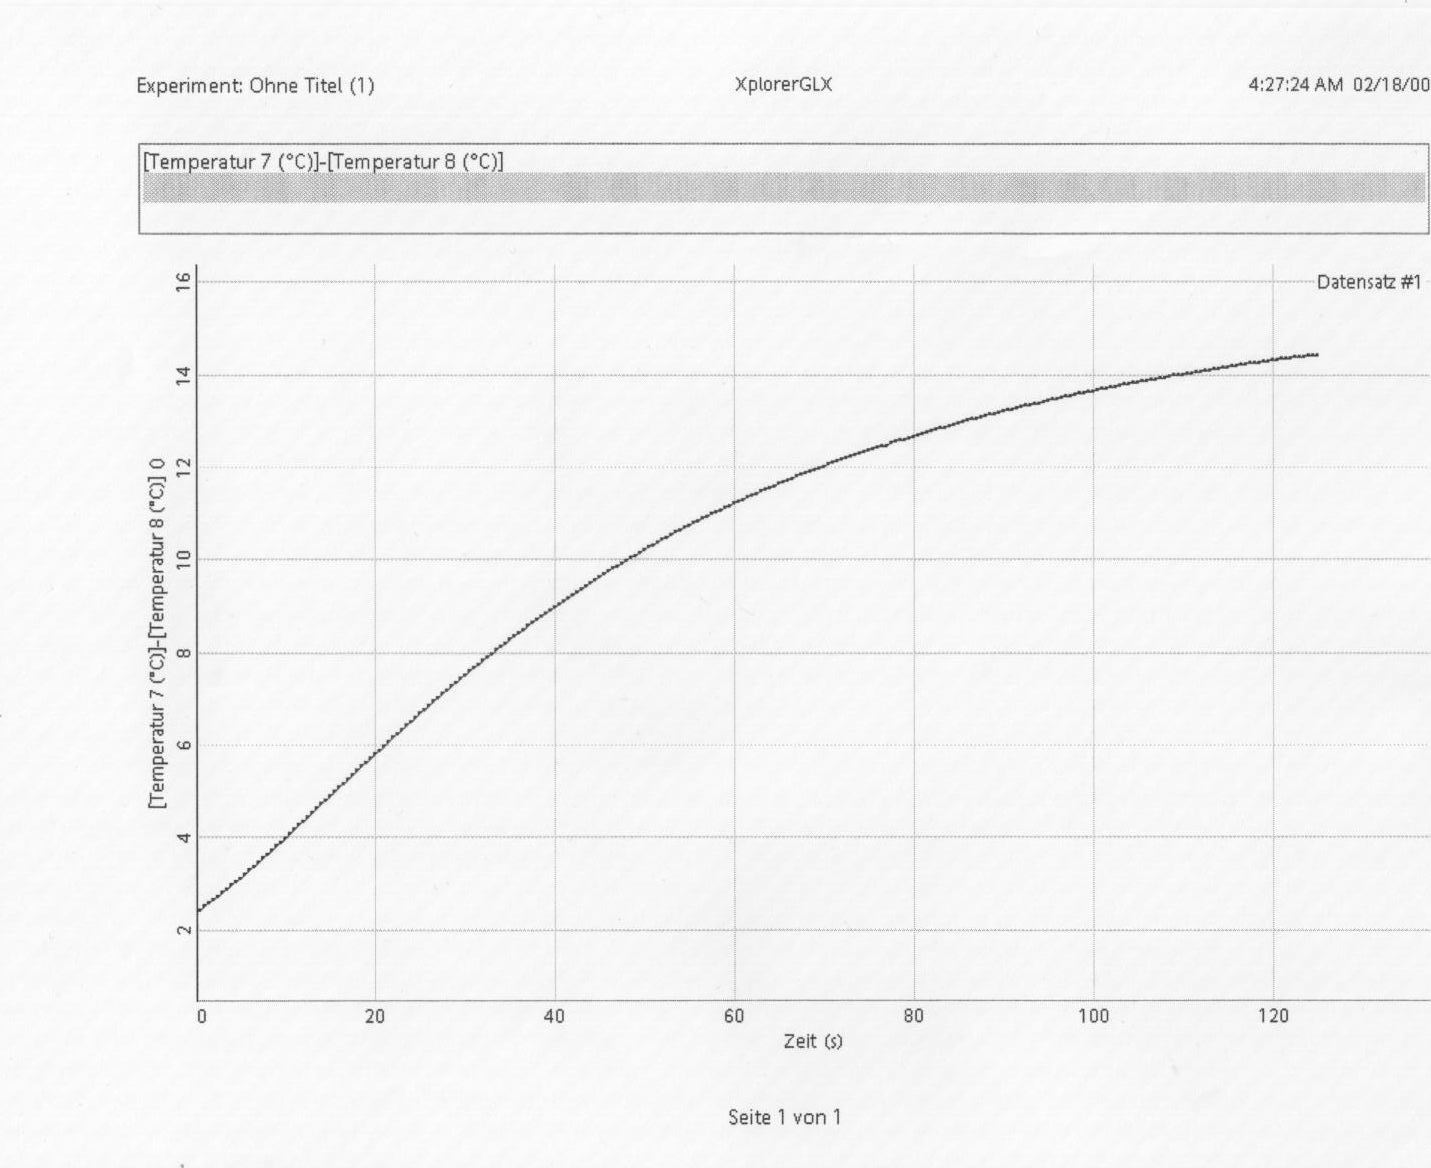
\includegraphics[width=0.7\textwidth]{data/t7minust8.JPEG}
  \caption{Verlauf der Temperaturdifferenz des fernen und des nahen Thermoelements am Edelstahlstab
   in Abhängigkeit von der Zeit}
  \label{fig:Stahl_diff}
\end{figure}

Bei beiden Stäben steigt die Temperaturdifferenz zunächst stark an, flacht danach jedoch ab.
Beim Messingstab ist zudem ein Maximum und ein anschließendes Abfallen der Temperaturdifferenz
zu beobachten. Die Temperaturdifferenz ist insgesamt bei dem Edelstahlstab größer.
Daraus lässt sich schließen, dass Messing die Wärme besser leitet und sich somit
homogener erhitzt als Edelstahl.


Nun soll für den breiten Messingstab und für den Edelstahlstab der Wärmestrom
zu fünf verschiedenen Zeiten bestimmt werden. Dafür wird die jeweilige Temperaturdifferenz
zum jeweiligen Zeitpunkt aus den Abbildungen \ref{fig:Messing_diff} und
\ref{fig:Stahl_diff} abgelesen. Zur Berechnung wird Gleichung \eqref{eqn:waerme}
verwendet und die Differenzialquotienten als Differenzenquotienten diskretisiert. Die Werte für die Querschnittsfläche $A$ der Stäbe können der Versuchsanleitung
\cite{Versuchsanleitung} entnommen werden. Die Werte für die Wärmeleitfähigkeit $\kappa$ wurden in der
Literatur (ZITAT) nachgeschlagen. Der Abstand zwischen den beiden Thermoelementen
wird durch Messung zu $d=\SI{3.0}{\centi\meter}$ bestimmt. Die für die Rechnung verwendeten Werte sind:
\begin{align}
  \kappa_{\symup{Messing}} &= \SI{112}{\joule\per\meter\per\kelvin}\,, \nonumber\\
  A_{\symup{Messing}} &= \SI{48e-6}{\meter}\,, \nonumber\\
  \kappa_{\symup{Edelstahl}} &= \SI{45}{\joule\per\meter\per\kelvin}\,, \nonumber\\
  A_{\symup{Edelstahl}} &= \SI{48e-6}{\meter}\,. \nonumber
\end{align}
In Tabelle \ref{tab:waermestrom} sind die abgelesenen Werte und die daraus berechneten Werte
für den Wärmestrom zu finden.

\begin{table}
  \centering
  \caption{Abgelesene Werte für die Temperaturdifferenz $\Delta T$ am Messingstab und am Edelstahlstab
  in Abhängigkeit von der Zeit $t$ und die daraus berechneten Werte für den Wärmestrom
  $\Delta Q/\Delta t$}
  \label{tab:waermestrom}
  \begin{tabular}{c c c c c}
    \toprule
    $t/$s & $\Delta T_{21}/$K & $\frac{\Delta Q_{21}}{\Delta t}/$W & $\Delta T_{78}/$K & $\frac{\Delta Q_{78}}{\Delta t}/$W \\
    \midrule
    20  & 6,04  & -1,08 & 5,81  & -0,42 \\
    40  & 6,81  & -1,22 & 8,97  & -0,65 \\
    60  & 6,95  & -1,25 & 11,23 & -0,81 \\
    80  & 6,87  & -1,23 & 12,65 & -0,91 \\
    100 & 6,72  & -1,20 & 13,68 & -0,98 \\
    \bottomrule
  \end{tabular}
\end{table}


\subsection{Dynamische Methode}
\label{sec:auswertung_dynamisch}

Zur Auswertung der dynamischen Methode soll die Wärmeleitfähigkeit $\kappa$ von
Messing, Aluminium und Edelstahl nach Gleichung \eqref{eqn:kappa} bestimmt werden.
Dafür werden aus den angefertigten Graphen Werte für die jeweiligen Amplituden
$A_{\symup{nah}}$ und $A_{\symup{fern}}$, sowie für die Phasendifferenz $\Delta t$ abgelesen. Erneut wird für den Abstand der
Thermoelemente bei dieser Messreihe für alle Stäbe zu $\SI{3.0}{\centi\meter}$ bestimmt.
Die zusätzlich benötigten Werte für die Dichte $\rho$ und die spezifische Wärmekapazität $c$
der Legierungen und Metalle können der Versuchsanleitung entnommen werden. Die Graphen
finden sich in den Abbildungen \ref{fig:messing_welle} bis \ref{fig:edelstahl_welle}.

Für Messing wurden die Folgenden Werte verwendet:
\begin{align}
  \rho &= \SI{8520}{\kilo\gram\per\cubic\meter}\,, \nonumber\\
  c &= \SI{385}{\joule\per\kilo\gram\per\kelvin}\,, \nonumber\\
  \ln{\frac{A_{\symup{nah}}}{A_{\symup{fern}}}} &= 1,17 \pm 0,05 \,, \nonumber\\
  \Delta t &= \SI{15.8(11)}{\second} \,. \nonumber
\end{align}
Die zugrundeliegenden Messdaten können Tabelle \ref{tab:messing_welle} entnommen
werden. Die fehlerbehafteten Werte wurden dabei mit Gleichung \eqref{eqn:mean} gemittelt
und ihre Standardabweichungen mit Gleichung \eqref{eqn:std} berechnet.

\begin{figure}
  \centering
  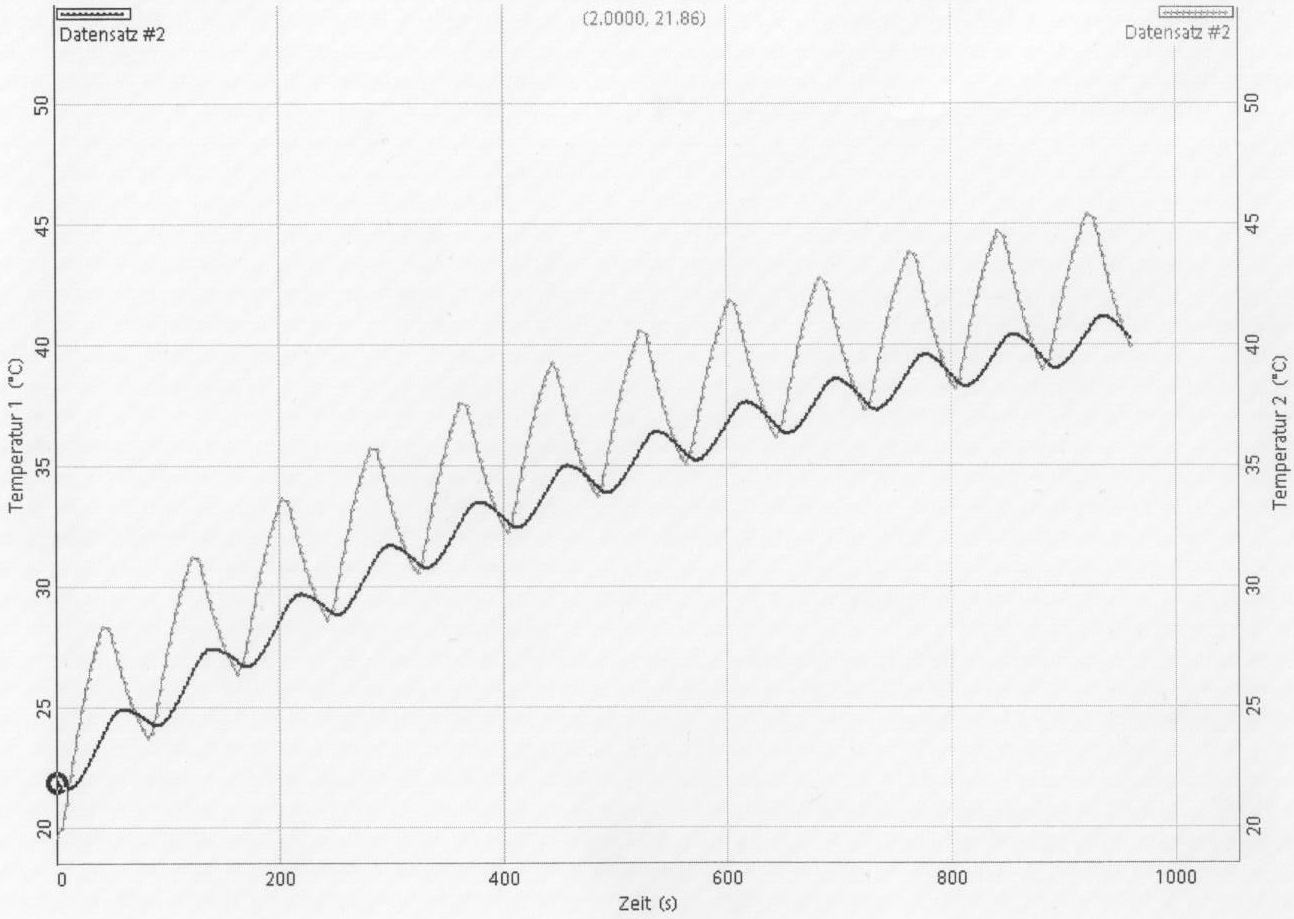
\includegraphics[width=0.7\textwidth]{data/t1undt2_welle.JPEG}
  \caption{Temperaturverlauf des Messingstabes am nahen Thermoelement (in der Abbildung dünn dargestellt)
  und am fernen Thermoelement (in der Abbildung dick dargestellt) in Abhängigkeit von der Zeit}
  \label{fig:messing_welle}
\end{figure}

\begin{table}
  \centering
  \caption{Abgelesene Werte für die Amplituden $A_{\symup{nah}}$ und $A_{\symup{fern}}$ der Temperaturen und
  ihrer Phasendifferenz am Messingstab und daraus berechnete Logarithmen der Amplitudenquotienten}
  \label{tab:messing_welle}
  \begin{tabular}{c c c c}
    \toprule
     $A_{\symup{nah}}/$K  & $A_{\symup{fern}}/$K & $\ln\Bigl(\frac{A_{\symup{nah}}}{A_{\symup{fern}}}\Bigr)$ & $\Delta t$ \\
    \midrule
    6,6 & 1,9 & 1,26  & 16  \\
    6,2 & 2,1 & 1,08  & 16  \\
    6,1 & 1,9 & 1,17  & 14  \\
    6,1 & 2,0 & 1,12  & 17  \\
    6,3 & 1,9 & 1,20  & 18  \\
    6,3 & 1,9 & 1,20  & 15  \\
    6,3 & 2,0 & 1,15  & 16  \\
    6,3 & 2,0 & 1,15  & 14  \\
    6,1 & 1,9 & 1,17  & 16  \\
    6,2 & 1,9 & 1,18  & 16  \\
    6,3 & 1,9 & 1,20  & 16  \\
    \bottomrule
  \end{tabular}
\end{table}

Wird nun die Wärmeleitfähigkeit $\kappa$ gemäß \eqref{eqn:kappa} berechnet, so ergibt sich
\begin{align}
  \kappa_{\symup{Messing}} &= \SI{80(6)}{\watt\per\meter\per\kelvin}\,.\nonumber
\end{align}
Dabei muss die Gauß'sche Fehlerfortpflanzung mittels Gleichung \eqref{eqn:gaussfehler}
berücksichtigt werden.
Der Literaturwert für die Wärmeleitfähigkeit von Messing liegt bei
$\kappa_{\symup{Messing,lit}}=\SI{112}{\watt\per\meter\per\kelvin}$ \cite{Wärmeleitfähigkeit1}.
Die Abweichung der Messung entspricht also 28,57\%. Je nach Legierung kann
jedoch auch der Wert für die Wärmeleitfähigkeit von Messing variieren, sodass auch Werte von
$\kappa_{\symup{Messing}} = \SI{81}{\watt\per\meter\per\kelvin}$ \cite{Wärmeleitfähigkeit2}
möglich sind.




Für Aluminium ergeben sich die Werte
\begin{align}
  \rho &= \SI{2800}{\kilo\gram\per\cubic\meter}\,, \nonumber\\
  c &= \SI{830}{\joule\per\kilo\gram\per\kelvin}\,, \nonumber\\
  \ln{\frac{A_{\symup{nah}}}{A_{\symup{fern}}}} &= 0,73 \pm 0,03 \,, \nonumber\\
  \Delta t &= \SI{7.5(11)}{\second} \,.\nonumber
\end{align}
Sie wurden analog zu denen von Messing berechnet. Die zugehörigen Messdaten sind
in Tabelle \ref{tab:aluminium_welle} aufgelistet.

\begin{figure}
  \centering
  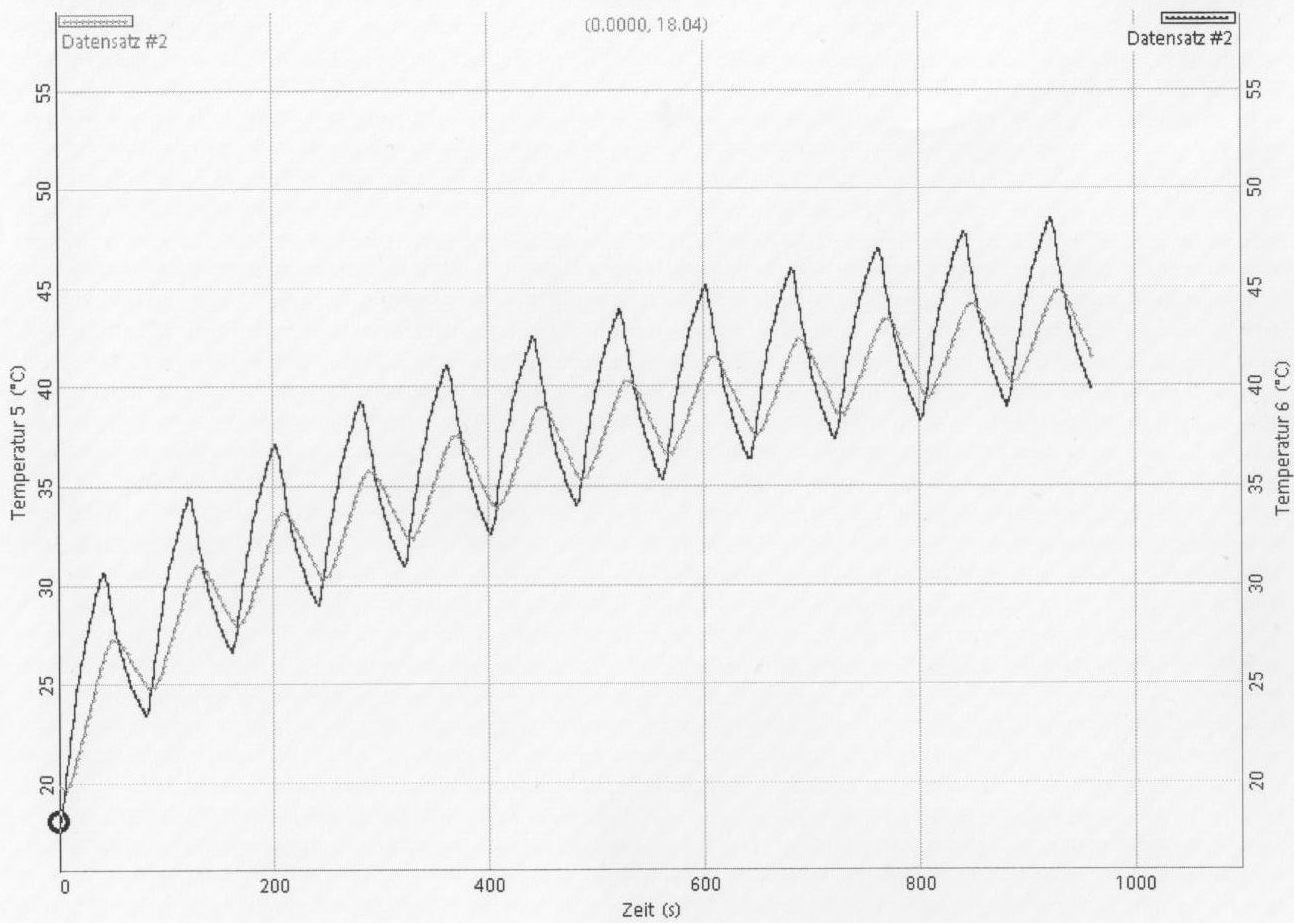
\includegraphics[width=0.7\textwidth]{data/t5undt6_welle.JPEG}
  \caption{Temperaturverlauf des Aluminiumstabes am nahen Thermoelement (in der Abbildung dick dargestellt)
  und am fernen Thermoelement (in der Abbildung dünn dargestellt) in Abhängigkeit von der Zeit}
  \label{fig:aluminium_welle}
\end{figure}

\begin{table}
  \centering
  \caption{Abgelesene Werte für die Amplituden $A_{\symup{nah}}$ und $A_{\symup{fern}}$ der Temperaturen und
  ihrer Phasendifferenz am Aluminiumstab und daraus berechnete Logarithmen der Amplitudenquotienten}
  \label{tab:aluminium_welle}
  \begin{tabular}{c c c c}
    \toprule
     $A_{\symup{nah}}/$K  & $A_{\symup{fern}}/$K & $\ln\Bigl(\frac{A_{\symup{nah}}}{A_{\symup{fern}}}\Bigr)$ & $\Delta t$ \\
    \midrule
    10  	& 5,2  &  0,65 &  7 \\
    9,4	  & 4,7	 &  0,69 &  7 \\
    9,3	  & 4,5	 &  0,73 &  7 \\
    9,4	  & 4,6	 &  0,71 &  9 \\
    9,3	  & 4,4	 &  0,75 &  8 \\
    9,3	  & 4,3	 &  0,77 &  6 \\
    9,2	  & 4,3	 &  0,76 &  6 \\
    9,2	  & 4,4	 &  0,74 &  7 \\
    9,1	  & 4,4	 &  0,73 &  9 \\
    9,1	  & 4,4	 &  0,73 &  9 \\
    9,1	  & 4,4	 &  0,73 &  7 \\
    \bottomrule
  \end{tabular}
\end{table}
Die Wärmeleitfähigkeit ergibt sich dann ebenfalls nach Gleichung \eqref{eqn:kappa}
und \eqref{eqn:gaussfehler} zu
\begin{align}
  \kappa_{\symup{Aluminium}} &= \SI{193(29)}{\watt\per\meter\per\kelvin}\,.\nonumber
\end{align}
Hier ist auffällig, dass der Fehler sehr groß ist.
Der Literaturwert für die Wärmeleitfähigkeit von Aluminium ist
$\kappa_{\symup{Aluminium}} = \SI{220}{\watt\per\meter\per\kelvin}$ \cite{Wärmeleitfähigkeit1}. Die relative
Abweichung beträgt 12,27\%.


Für Edelstahl lassen sich folgende Werte finden:
\begin{align}
  \rho &= \SI{8000}{\kilo\gram\per\cubic\meter}\,, \nonumber\\
  c &= \SI{400}{\joule\per\kilo\gram\per\kelvin}\,, \nonumber\\
  \ln{\frac{A_{\symup{nah}}}{A_{\symup{fern}}}} &= 1,96\pm 0,04 \,, \nonumber\\
  \Delta t &= \SI{7.5(11)}{\second} \,.\nonumber
\end{align}
Sie wurden ebenfalls analog zu denen von Messing berechnet. Die Messdaten zu dieser Messreihe
finden sich in Tabelle \ref{tab:edelstahl_welle}.

\begin{figure}
  \centering
  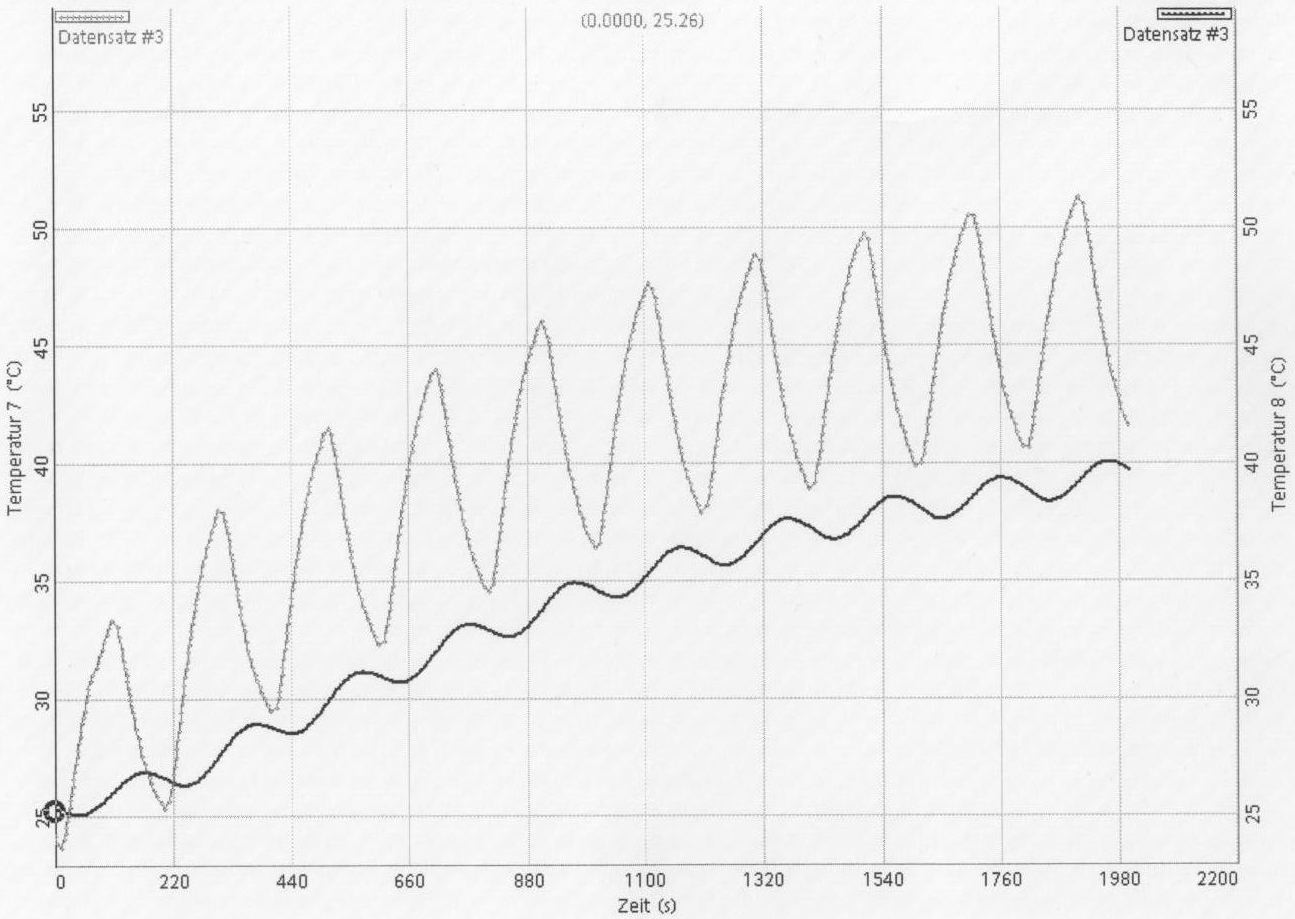
\includegraphics[width=0.7\textwidth]{data/t7undt8_welle.JPEG}
  \caption{Temperaturverlauf des Edelstahlstabes am nahen Thermoelement (in der Abbildung dünn dargestellt)
  und am fernen Thermoelement (in der Abbildung dick dargestellt) in Abhängigkeit von der Zeit}
  \label{fig:edelstahl_welle}
\end{figure}

\begin{table}
  \centering
  \caption{Abgelesene Werte für die Amplituden $A_{\symup{nah}}$ und $A_{\symup{fern}}$ der Temperaturen und
  ihrer Phasendifferenz am Edelstahlstab und daraus berechnete Logarithmen der Amplitudenquotienten}
  \label{tab:edelstahl_welle}
  \begin{tabular}{c c c c}
    \toprule
     $A_{\symup{nah}}/$K  & $A_{\symup{fern}}/$K & $\ln\Bigl(\frac{A_{\symup{nah}}}{A_{\symup{fern}}}\Bigr)$ & $\Delta t$ \\
    \midrule
    9	    & 1.2 &	2.01  & 55 \\
    10.8	& 1.5 & 1.97	& 64  \\
    10.5  &	1.5	& 1.95  & 59  \\
    10.6	& 1.4	& 2.02  & 64 \\
    10.5	& 1.6	& 1.88  & 57 \\
    10.5	& 1.5	& 1.95  & 57 \\
    10.5	& 1.5	& 1.95  & 65 \\
    10.5	& 1.5	& 1.95  & 58 \\
    10.3  &	1.5	& 1.93  & 59  \\
    \bottomrule
  \end{tabular}
\end{table}

Auch hier ergibt sich die Wärmeleitfähigkeit nach Gleichung \eqref{eqn:kappa}
und \eqref{eqn:gaussfehler} zu
\begin{align}
  \kappa_{\symup{Edelstahl}} = \SI{12.3(08)}{\watt\per\meter\per\kelvin}\,.\nonumber
\end{align}
Der Literaturwert ist $\kappa_{\symup{Edelstahl}} = \SI{15}{\watt\per\meter\per\kelvin}$
\cite{Wärmeleitfähigkeit3}.
Die relative Abweichung beträgt hier 18,00\%.
